\section{Diagramma delle classi}
\label{sec:diagramma delle classi}
Durante lo sviluppo della parte back-end, sono state create diverse classi di supporto allo sviluppo del componente. In figura \ref{fig:UMLSD}, diagramma delle classi (UML), è possibile vedere tutte le classi che entrano in gioco per la realizzazione dell'applicativo.
\\L'applicativo sviluppato ha come punto di partenza (\textit{main}) un Job di Spark. Dalla documentazione ufficiale un job di Spark è un calcolo parallelo composto da più attività che vengono generate in risposta a un'azione \cite{spark:job}. In parole povere, è una serie di istruzioni che vengono eseguite in parallelo su più macchine, ottimizzando i tempi di risposta dell'applicativo. 
\\I passi fondamentali per creare un Job di Spark sono:
\begin{itemize}
\item \textbf{Caricare le librerie}: Immettere nel proprio \textit{classpath} le librerie di Spark.
\item \textbf{Inizializzare il contesto di Spark}: La prima operazione di codice da effettuare è quella di inizializzare lo \textit{SparkContext}, in cui comunica la locazione dei cluster da utilizzare ed altre impostazioni quali il numero, i driver di connessione, etc.
\item \textbf{Parallelizzare le collezioni di dati}: I dati di input devono essere parallelizzati tramite il metodo di SparkContext \textit{parallelize}.
Con questo metodo gli elementi della collezione vengono copiati per formare un set di dati distribuito che può essere gestito in parallelo. I dati parallelizzati diventano RDD.
\item \textbf{Operazioni sugli RDD}: Ai dati parallelizzati si applicano le principali operazioni di Spark come map, filter, reduce, etc.
\end{itemize}
Nell'applicativo questi passi sono svolti dalla classe principale che contiene il main: \textit{"App"}. La classe in questione però utilizza delle classi create ad-hoc per gestire al meglio alcuni aspetti. Di seguito sono riportate le principali classi con una breve descrizione delle loro funzionalità: 
\begin{figure}[H]
	\centering
	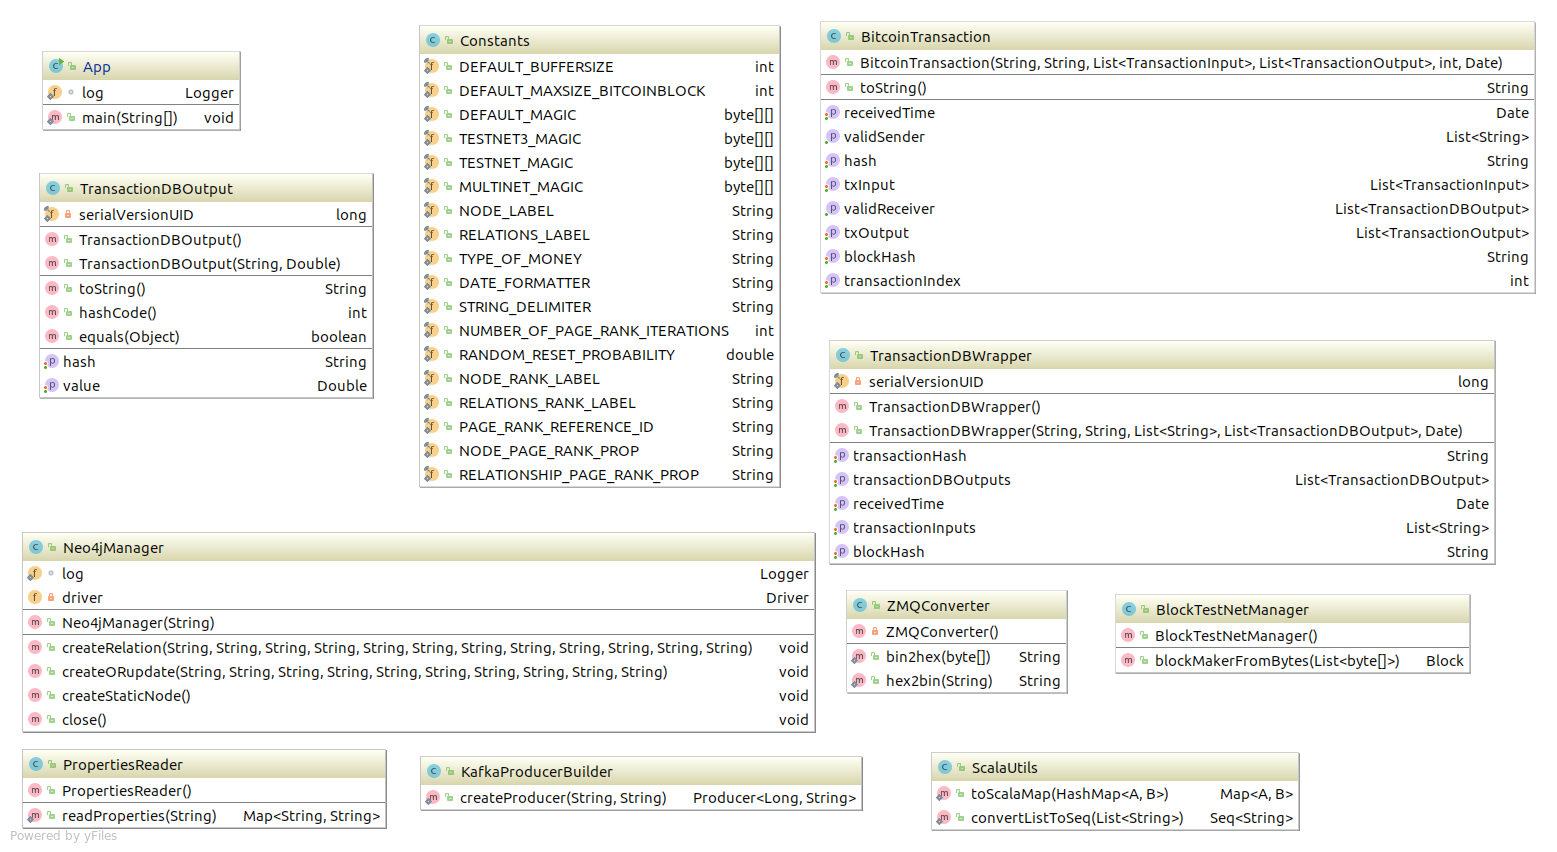
\includegraphics[width=\textwidth, height=0.45\textheight, keepaspectratio]{images/AppUML.png}
	\caption{UML delle classi (Sistema distribuito).}
	\label{fig:UMLSD}
\end{figure}
\begin{itemize}
\item \textbf{\textit{App}}: Questa classe è il fulcro di tutto l'applicativo. Infatti, è colei che si occupa della creazione del Job di Spark, del salvataggio nelle periferiche esterne e della messa a disposizione dei dati elaborati. In particolare, la classe App è la prima ad essere eseguita lanciando il Job di Spark Streaming che costantemente attende dati provenienti da blockchain. Ottenuti i dati, li invia al cluster di Spark che li elabora li salva sul filesystem Hadoop e nella base dati Neo4j. Questo primo passaggio è poi accompagnato dall'analisi dello stato delle transazioni esistenti, effettuato tramite la libreria GraphX, la quale applica l'algoritmo del Page Rank sui nodi presenti in Neo4j. Terminata questa fase, le ultime righe di codice creano un collegamento con Kafka per inviare i dati sui topic. 
\item \textbf{\textit{Constants}}: Questa classe è utilizza per il salvataggio ed il recupero delle costanti come gli IP delle macchine utilizzate (hadoop, kafka, neo4j), nomi dei nodi per il database etc.
\item  \textbf{\textit{BitcoinTransaction}}: La classe in questione viene utilizzata da App per creare una struttura dati in memoria che semplifica la gestione delle transazioni. Infatti, essa rappresenta l'astrazione di una transazione Bitcoin.
\item  \textbf{\textit{TransactionDBWrapper}}: Come dice il nome, questa classe è un wrapper (contenitore) per le transazioni inviate a Neo4j.
\item  \textbf{\textit{TransactionDBOutput}}: Analogamente alla precedente, questa classe è utilizzata per avere una idea di nodo quando vengono recuperate le transazioni dal database.
\item  \textbf{\textit{Neo4jManager}}: La classe Neo4jManager è fondamentale per il salvataggio dei dati in Neo4j. Infatti, si occupa della creazione di una connessione con il database, delle query da eseguire su di esso e dell'estrazione dei dati.
\end{itemize}
Sul fronte visualizzazione il discorso cambia. Il linguaggio Javascript infatti, difficilmente utilizza il paradigma ad oggetti evitando quindi di creare classi. In contrapposizione però utilizza procedure che si attivano in risposta ad una azione o ad una specifica richiesta. Per questo motivo creare un diagramma delle classi non avrebbe senso.
\\ In Blockchain explorer quindi sono stati creati una serie di file Javscript che vengono richiamati all'occorrenza dal framework NodeJS. I file in questione, figura \ref{fig:rootWebApp}, sono i componenti principali che compongono la webapp. Occorre però fare una divisione del Javascript che viene eseguito lato client e quello lato Server. Infatti tutti i file contenuti nella cartella \textit{public} sono script che vengono eseguiti solo dai browser dei client, poiché sono integrati nell'HTML che il server genera dinamicamente. I restanti file invece sono eseguiti dal motore di Chrome V8 tramite NodeJS solo sul server.
\begin{figure}[H]
	\centering
	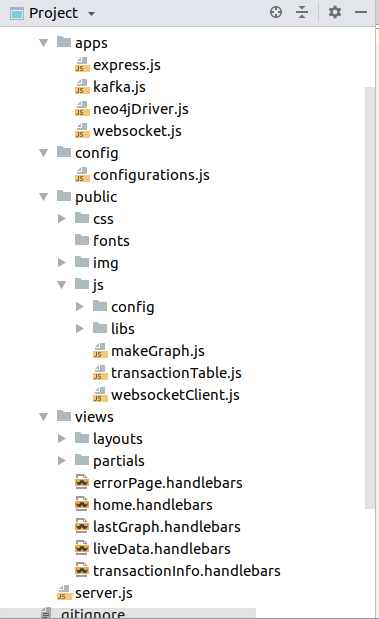
\includegraphics[width=0.5\textwidth, height=0.45\textheight, keepaspectratio]{images/webAppRoot.png}
	\caption{Alberatura file di Blochchain Explorer.}
	\label{fig:rootWebApp}
\end{figure}
Ogni file ha un funzione specifica definita di seguito:
\begin{itemize}
\item  \textbf{\textit{server.js}}: Questo è un file di inizializzazione, nella quale viene inizializzato il server in ascolto su di una porta e caricato il framework Express. Esso rappresenta dunque il punto iniziale di tutte le richieste che verranno smistate.
\item  \textbf{\textit{configuration.js}}: E' un file che contiene le principali costanti dell'applicativo come la porta su cui far partire il server, la porta della websocket ed altri settaggi utili per il funzionamento dell'applicazione.
\item  \textbf{\textit{express.js}}: Questo file è il cuore della webapp. Essa contiene tutte le \textit{route} possibili. Infatti, contiene tutta la catena di funzioni per gestire una richiesta da parte dei client. In altre parole, in questo file sono fatte le associazioni tra path richiesto dal client e callback eseguita in risposta. In questo file troviamo il codice che viene eseguito ad ogni richiesta client, dalla visualizzazione del grafo alle ultime transazioni. Le callback, per restituire ai client una valida risposta, richiamano a loro volta funzioni provenienti da altri file.
\item  \textbf{\textit{kafka.js}}: Contiene l'implementazione del Kafka Subscriber, quindi si occupa della connessione a Kafka ed alla ricezione dei dati da parte del topic.
\item  \textbf{\textit{neo4jDriver.js}}: Analogamente a Neo4jManager, viene usato per la connessione ed il recupero dei dati presenti in base dati Neo4j. In particolare, utilizza il linguaggio Cypher per ottenere i risultati dal database. 
\item  \textbf{\textit{websocket.js}}: Questo script crea un server WebSocket per permettere ai vari client di ricevere le transazioni in real-time tramite protocollo WebSocket.
\item  \textbf{\textit{Cartella views}}: In questa cartella sono presenti tutti i template utilizzati dal sito. Infatti, contiene tutti i file con estensione \textit{.handlebars} utili al framework per creare pagine HTML dinamiche. All'interno di questi template sono linkati tutti gli script e i fogli di stile presenti nella cartella \textit{public}.
\item  \textbf{\textit{Cartella public}}: Questa cartella contiene tutte le risorse statiche che vengono caricate ed eseguite dai browser. I file Javascript presenti in questa cartella stabiliscono una connessione con il server tramite WebSocket, disegnano il grafo delle transazioni dinamicamente e creano le tabelle all'interno del sito.
\\Gli script di particolare importanza sono:
\begin{itemize}
\item  \textbf{\textit{MakeGraph.js}}: Lo script contenuto in questo file, utilizza la libreria D3.js per disegnare i grafi delle transazioni presenti sul sito.
\item  \textbf{\textit{transactionTable.js}}: Questo file contiene lo script che genera le tabelle. Grazie all'utilizzo della libreria DataTable riesce a disegnare in modo efficiente tabelle anche di grandi dimensioni.
\item  \textbf{\textit{websocketClient.js}}: Come dice il nome, questo file permette la connessione col server WebSocket istanziato da NodeJS.
\end{itemize}
\end{itemize}